\begin{tomtat}
	\begin{minipage}[t]{0.3\textwidth}
		\vspace{0pt}
		\begin{tomtat}
			\begin{center}
				\textbf{ĐỀ 13}
			\end{center}
			
		\end{tomtat}
	\end{minipage}
	\hfill
	\begin{minipage}[t]{0.5\textwidth}
		\vspace{0pt}
		\begin{tomtat}
			\begin{center}
				\includegraphics[scale=0.08]{images/13}
			\end{center}
		\end{tomtat}
	\end{minipage}
\end{tomtat}
\textbf{I. PHẦN TRẮC NGHIỆM}
\begin{ex}
	Giá trị của biểu thức $\sqrt[3]{125} \cdot \sqrt[3]{27} - \sqrt[3]{64}$ bằng:
	\choice{9}{10}{11}{12}
	\loigiai{
		Ta có:
		$\sqrt[3]{125} = 5$ (vì $5^3 = 125$)
		$\sqrt[3]{27} = 3$ (vì $3^3 = 27$)
		$\sqrt[3]{64} = 4$ (vì $4^3 = 64$)
		Vậy, giá trị của biểu thức là:
		\begin{align*}
			\sqrt[3]{125} \cdot \sqrt[3]{27} - \sqrt[3]{64} &= 5 \cdot 3 - 4 \\
			&= 15 - 4 \\
			&= 11
		\end{align*}
		\\ \textbf{ĐÁP ÁN C}
	}
\end{ex}

\begin{ex}
	Điểm $P(-1;-2)$ thuộc đồ thị hàm số $y=mx^2$ khi $m$ bằng:
	\choice{2}{-2}{4}{-4}
	\loigiai{
		Đồ thị hàm số $y=mx^2$ đi qua điểm $P(-1;-2)$ có nghĩa là khi $x=-1$ thì $y=-2$.
		Thay $x=-1$ và $y=-2$ vào phương trình hàm số, ta được:
		\begin{align*}
			-2 &= m(-1)^2 \\
			-2 &= m \cdot 1 \\
			m &= -2
		\end{align*}
		Vậy giá trị của $m$ là -2.
		\\ \textbf{ĐÁP ÁN B}
	}
\end{ex}

\begin{ex}
	Điều kiện xác định của biểu thức $\sqrt{3x+1}$ là:
	\choice{$x \le -\frac{1}{3}$}{$x \ne -3$}{$x \ge -\frac{1}{3}$}{$x \ge 0$}
	\loigiai{
		Biểu thức $\sqrt{3x+1}$ xác định khi biểu thức dưới dấu căn không âm.
		Tức là $3x+1 \ge 0$.
		\begin{align*}
			3x+1 &\ge 0 \\
			3x &\ge -1 \\
			x &\ge -\frac{1}{3}
		\end{align*}
		Vậy điều kiện xác định của biểu thức là $x \ge -\frac{1}{3}$.
		\\ \textbf{ĐÁP ÁN C}
	}
\end{ex}

\begin{ex}
	Cho tam giác MNP vuông tại M. Khi đó $\cos\widehat{MNP}$ là:
	\choice{$\frac{MP}{NP}$}{$\frac{MN}{NP}$}{$\frac{MN}{MP}$}{$\frac{MP}{NM}$}
	\loigiai{
		Trong tam giác MNP vuông tại M:
		Góc $\widehat{MNP}$ chính là góc N.
		Theo định nghĩa tỉ số lượng giác cosin trong tam giác vuông, ta có:
		$$ \cos N = \cos\widehat{MNP} = \frac{\text{cạnh kề}}{\text{cạnh huyền}} = \frac{MN}{NP} $$
		\\ \textbf{ĐÁP ÁN B}
	}
\end{ex}

\begin{ex}
	Nghiệm của Pt: $-2(3-x)=-10$.
	\choice{$x=8$}{$x=-8$}{$x=2$}{$x=-2$}
	\loigiai{
		Ta giải phương trình:
		\begin{align*}
			-2(3-x) &= -10 \\
			3-x &= \frac{-10}{-2} \\
			3-x &= 5 \\
			-x &= 5-3 \\
			-x &= 2 \\
			x &= -2
		\end{align*}
		Vậy nghiệm của phương trình là $x=-2$.
		\\ \textbf{ĐÁP ÁN D}
	}
\end{ex}

\begin{ex}
	Diện tích của mặt cầu có bán kính $r=2 \text{ cm}$ bằng:
	\choice{$16\pi \text{ cm}^2$}{$8\pi \text{ cm}^2$}{$4\pi \text{ cm}^2$}{$\frac{32}{3}\pi \text{ cm}^2$}
	\loigiai{
		Diện tích mặt cầu được tính bằng công thức: $S = 4\pi r^2$.
		Với $r=2 \text{ cm}$:
		\begin{align*}
			S &= 4\pi (2)^2 \\
			&= 4\pi \cdot 4 \\
			&= 16\pi (\text{cm}^2)
		\end{align*}
		\\ \textbf{ĐÁP ÁN A}
	}
\end{ex}

\begin{ex}
	Đo chiều cao (đơn vị cm) của học sinh lớp 9A ở một trường THCS trên địa bàn tỉnh Thanh Hóa ta có bảng tần số ghép nhóm như sau:
	\begin{center}
		\begin{tabular}{|l|c|c|c|c|}
			\hline
			[150;158) & [158;161) & [161;164) & [164;167) \\
			\hline
			5 & 12 & 15 & 8 \\
			\hline
		\end{tabular}
	\end{center}
	Khi đó tỉ lệ học sinh có chiều cao từ 158cm đến dưới 161cm là:
	\choice{12,5\%}{30\%}{37,5\%}{20\%}
	\loigiai{
		Tổng số học sinh được đo là $N = 5 + 12 + 15 + 8 = 40$ học sinh.
		Số học sinh có chiều cao từ 158cm đến dưới 161cm (nhóm [158;161)) là $n_{[158;161)} = 12$ học sinh.
		Tỉ lệ học sinh có chiều cao từ 158cm đến dưới 161cm là:
		$$ f = \frac{n_{[158;161)}}{N} \times 100\% $$
		$$ f = \frac{12}{40} \times 100\% $$
		$$ f = \frac{3}{10} \times 100\% = 0,3 \times 100\% = 30\% $$
		\\ \textbf{ĐÁP ÁN B}
	}
\end{ex}
\begin{ex} % Câu 8 (từ ảnh mới)
	Gieo hai đồng xu cân đối và đồng chất một lần. Tính xác suất sao cho hai đồng xu xuất hiện mặt giống nhau.
	\choice{0}{$\frac{1}{4}$}{1}{$\frac{1}{2}$}
	\loigiai{
		Ký hiệu mặt sấp là S, mặt ngửa là N.
		Khi gieo hai đồng xu cân đối và đồng chất một lần, tập hợp tất cả các kết quả có thể xảy ra (không gian mẫu $\Omega$) là:
		$\Omega = \{ \text{(S,S)}, \text{(S,N)}, \text{(N,S)}, \text{(N,N)} \}$.
		Trong đó, phần tử thứ nhất là kết quả của đồng xu thứ nhất, phần tử thứ hai là kết quả của đồng xu thứ hai.
		Số phần tử của không gian mẫu là $n(\Omega) = 4$.
		
		Gọi A là biến cố "hai đồng xu xuất hiện mặt giống nhau".
		Tập hợp các kết quả thuận lợi cho biến cố A là:
		$A = \{ \text{(S,S)}, \text{(N,N)} \}$.
		Số phần tử của biến cố A là $n(A) = 2$.
		
		Xác suất của biến cố A là:
		$$ P(A) = \frac{n(A)}{n(\Omega)} = \frac{2}{4} = \frac{1}{2} $$
		\\ \textbf{ĐÁP ÁN D}
	}
\end{ex}
\newpage
\textbf{II. PHẦN TỰ LUẬN}
\begin{ex} % Câu 9
	(1,0 điểm): Rút gọn biểu thức P, biết: $C=\frac{2\sqrt{x}+4}{x-4}-\frac{3}{2-\sqrt{x}}$ với $x \ge 0, x \ne 4$. 
	% Lưu ý: Đề bài ghi là rút gọn P, nhưng biểu thức lại là C. Giả sử là rút gọn C.
	\loigiai{
		Với $x \ge 0, x \ne 4$, ta có $x-4 = (\sqrt{x}-2)(\sqrt{x}+2)$ và $2-\sqrt{x} = -(\sqrt{x}-2)$.
		\begin{align*}
			C &= \frac{2\sqrt{x}+4}{(\sqrt{x}-2)(\sqrt{x}+2)} - \frac{3}{-(\sqrt{x}-2)} \\
			&= \frac{2(\sqrt{x}+2)}{(\sqrt{x}-2)(\sqrt{x}+2)} + \frac{3}{\sqrt{x}-2} \\
			&= \frac{2}{\sqrt{x}-2} + \frac{3}{\sqrt{x}-2} \\
			&= \frac{2+3}{\sqrt{x}-2} \\
			&= \frac{5}{\sqrt{x}-2}
		\end{align*}
		Vậy $C = \frac{5}{\sqrt{x}-2}$.
	}
\end{ex}

\begin{ex} % Câu 10
	(1,0 điểm): Giải hệ phương trình: $\begin{cases} 2x+y=3 \\ x-y=6 \end{cases}$.
	\loigiai{
		Ta có hệ phương trình:
		$$ \begin{cases} 2x+y=3 & (1) \\ x-y=6 & (2) \end{cases} $$
		Cộng vế theo vế của phương trình (1) và phương trình (2), ta được:
		\begin{align*}
			(2x+y) + (x-y) &= 3+6 \\
			3x &= 9 \\
			x &= 3
		\end{align*}
		Thay $x=3$ vào phương trình (2):
		\begin{align*}
			3-y &= 6 \\
			-y &= 6-3 \\
			-y &= 3 \\
			y &= -3
		\end{align*}
		Vậy nghiệm của hệ phương trình là $(x;y) = (3;-3)$.
	}
\end{ex}

\begin{ex} % Câu 11
	(1 điểm): Biết phương trình: $x^2-5x+3=0$ có 2 nghiệm $x_1, x_2$. Không giải phương trình, hãy tính giá trị của biểu thức: $P=5x_1^2+5x_2^2-x_1x_2+1$.
	\loigiai{
		Phương trình đã cho là $x^2-5x+3=0$.
		Đây là phương trình bậc hai có dạng $ax^2+bx+c=0$ với $a=1, b=-5, c=3$.
		Ta tính biệt thức $\Delta = b^2-4ac = (-5)^2 - 4(1)(3) = 25 - 12 = 13$.
		Vì $\Delta = 13 > 0$ nên phương trình có hai nghiệm phân biệt $x_1, x_2$.
		
		Theo hệ thức Vi-ét, ta có:
		$$ \begin{cases} 
			x_1+x_2 = \dfrac{-b}{a} = \dfrac{-(-5)}{1} = 5 \\ 
			x_1x_2 = \dfrac{c}{a} = \dfrac{3}{1} = 3 
		\end{cases} $$
		Ta cần tính giá trị của biểu thức $P=5x_1^2+5x_2^2-x_1x_2+1$.
		Biến đổi $x_1^2+x_2^2 = (x_1+x_2)^2 - 2x_1x_2$.
		Vậy,
		\begin{align*}
			P &= 5((x_1+x_2)^2 - 2x_1x_2) - x_1x_2 + 1 \\
			&= 5(x_1+x_2)^2 - 10x_1x_2 - x_1x_2 + 1 \\
			&= 5(x_1+x_2)^2 - 11x_1x_2 + 1
		\end{align*}
		Thay giá trị $x_1+x_2 = 5$ và $x_1x_2 = 3$ vào biểu thức $P$:
		\begin{align*}
			P &= 5(5)^2 - 11(3) + 1 \\
			&= 5(25) - 33 + 1 \\
			&= 125 - 33 + 1 \\
			&= 92 + 1 \\
			&= 93
		\end{align*}
		Vậy giá trị của biểu thức $P$ là 93.
	}
\end{ex}

\begin{ex} % Câu 12
	Tung đồng thời hai con xúc xắc đồng chất. Tính xác suất của biến cố "tổng số chấm xuất hiện trên hai con xúc xắc bằng 9".
	\loigiai{
		Tập hợp tất cả các kết quả có thể xảy ra khi tung đồng thời hai con xúc xắc (không gian mẫu $\Omega$) là các cặp (Xúc xắc 1, Xúc xắc 2):
		$n(\Omega) = 6 \times 6 = 36$.
		(Liệt kê đầy đủ sẽ có 36 cặp từ (1,1) đến (6,6)).
		
		Tập hợp các kết quả thuận lợi cho biến cố A: "tổng số chấm xuất hiện trên hai con xúc xắc bằng 9" là:
		$A = \{ (3,6), (4,5), (5,4), (6,3) \}$.
		Số kết quả thuận lợi cho biến cố A là $n(A) = 4$.
		
		Xác suất của biến cố A là:
		$$ P(A) = \frac{n(A)}{n(\Omega)} = \frac{4}{36} = \frac{1}{9} $$
	}
\end{ex}

\begin{ex} % Câu 13
	Một quyển sách Toán có giá bìa 30000 đồng, đang được giảm giá 5\%. Một quyển sách Văn có giá bìa 40000 đồng, đang được giảm giá 10\%. Trong thời gian giảm giá, nhà sách đó bán được tất cả 120 quyển sách Văn và Toán, thu được về số tiền là 3795000 đồng. Hỏi nhà sách đó đã bán được bao nhiêu quyển sách Văn, bao nhiêu quyển sách Toán?
	\loigiai{
		Giá sách Toán sau khi giảm giá 5\% là:
		$30000 \times (1 - 0,05) = 30000 \times 0,95 = 28500$ đồng.
		Giá sách Văn sau khi giảm giá 10\% là:
		$40000 \times (1 - 0,10) = 40000 \times 0,90 = 36000$ đồng.
		
		Gọi số quyển sách Toán đã bán được là $x$ (quyển).
		Gọi số quyển sách Văn đã bán được là $y$ (quyển).
		Điều kiện: $x, y \in \mathbb{N}^*$.
		
		Tổng số sách bán được là 120 quyển, nên ta có phương trình:
		$$ x + y = 120 \quad (1) $$
		Tổng số tiền thu được là 3795000 đồng, nên ta có phương trình:
		$$ 28500x + 36000y = 3795000 \quad (2) $$
		Chia cả hai vế của phương trình (2) cho 100:
		$$ 285x + 360y = 37950 $$
		Chia tiếp cho 15 (nếu có thể, hoặc để vậy giải):
		$285/15 = 19$, $360/15 = 24$, $37950/15 = 2530$.
		$$ 19x + 24y = 2530 \quad (2') $$
		
		Từ (1) $\Rightarrow y = 120 - x$. Thay vào $(2')$:
		\begin{align*}
			19x + 24(120-x) &= 2530 \\
			19x + 2880 - 24x &= 2530 \\
			-5x &= 2530 - 2880 \\
			-5x &= -350 \\
			x &= \frac{-350}{-5} \\
			x &= 70
		\end{align*}
		Thay $x=70$ vào $y = 120-x$:
		$y = 120 - 70 = 50$.
		Cả $x=70$ và $y=50$ đều thỏa mãn điều kiện.
		
		Vậy nhà sách đó đã bán được 70 quyển sách Toán và 50 quyển sách Văn.
	}
\end{ex}
\begin{ex} % Câu 13
Cho nửa đường tròn tâm $O$ đường kính $AB=2R$. Trên nửa mặt phẳng bờ $AB$, cùng phía với nửa đường tròn vẽ $Ax, By$ lần lượt là các tia tiếp tuyến của $(O)$ tại $A$ và $B$. Gọi $I$ là trung điểm của $AO$. Lấy hai điểm $P, Q$ nằm trên $Ax, By$ sao cho $\widehat{PIQ} = 90^\circ$. Gọi $H$ là hình chiếu vuông góc của $I$ lên $PQ$.
\begin{enumerate}
	\item Chứng minh tứ giác $APHI$ nội tiếp.
	\item Gọi $M, N$ lần lượt là giao điểm của $AH$ với $PI$ và $BH$ với $IQ$. Chứng minh $MN // AB$.
\end{enumerate}
	\loigiai{
		\begin{center}
		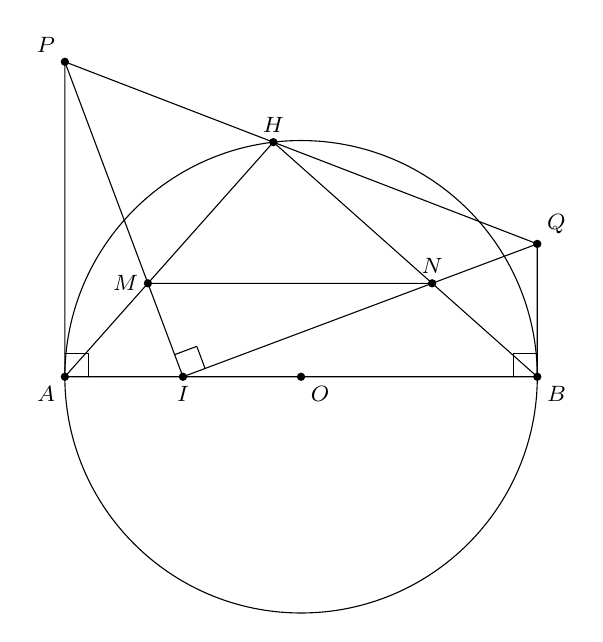
\begin{tikzpicture}[line join = round, line cap=round,>=stealth,font=\footnotesize,scale=1]
			\usetikzlibrary{calc,intersections,angles}
			
			% Khai báo hằng số
			\def\r{3} % r = 3cm
			\def\a{4} % a = 4
			
			% Định nghĩa tọa độ các điểm
			\coordinate (O) at (0,0);
			\coordinate (A) at (-\r,0);
			\coordinate (B) at (\r,0);
			\coordinate (I) at (-\r/2,0);
			\coordinate (P) at (-\r,\a);
			\coordinate (Q) at (\r,{3*\r^2/(4*\a)});
			
			% H là hình chiếu của I lên PQ
			\coordinate (H) at ($(P)!(I)!(Q)$);
			
			% M là giao điểm của AH và PI
			\path[name path=lineAH_M] (A) -- (H);
			\path[name path=linePI_M] (P) -- (I);
			\path[name intersections={of=lineAH_M and linePI_M, by=M}];
			
			% N là giao điểm của HB và IQ
			\path[name path=lineHB_N] (H) -- (B);
			\path[name path=lineIQ_N] (I) -- (Q);
			\path[name intersections={of=lineHB_N and lineIQ_N, by=N}];
			
			% Vẽ các đối tượng hình học
			\draw (O) circle (\r);          % Đường tròn (O;r)
			\draw (A) -- (B) -- (Q) -- (P) -- cycle; % Đa giác A-B-Q-P-A
			\draw (P) -- (I) -- (Q);        % Đường P-I-Q
			\draw (M) -- (N);               % Đoạn M-N
			\draw (A) -- (H) -- (B);        % Đường A-H-B
			
			% Tô màu cho các điểm (theo cấu trúc đầu tiên)
			\fill (O) circle (1.5pt);
			\fill (A) circle (1.5pt);
			\fill (B) circle (1.5pt);
			\fill (I) circle (1.5pt);
			\fill (P) circle (1.5pt);
			\fill (Q) circle (1.5pt);
			\fill (H) circle (1.5pt);
			\fill (M) circle (1.5pt);
			\fill (N) circle (1.5pt);
			
			% Đặt nhãn cho các điểm (theo cấu trúc đầu tiên)
			\node[below right] at (O) {$O$};
			\node[below left] at (A) {$A$};
			\node[below right] at (B) {$B$};
			\node[below] at (I) {$I$};
			\node[above left] at (P) {$P$};
			\node[above right] at (Q) {$Q$};
			\node[above] at (H) {$H$}; % Vị trí tương đối, có thể cần điều chỉnh
			\node[left] at (M) {$M$};   % Vị trí tương đối
			\node[above] at (N) {$N$};  % Vị trí tương đối
			
			% Ký hiệu các góc vuông
			% Góc PAO (vuông tại A)
			\pic[draw, angle radius=3mm]{right angle = P--A--O};
			% Góc QBA (vuông tại B)
			\pic[draw, angle radius=3mm]{right angle = Q--B--A};
			% Góc PIQ (vuông tại I)
			\pic[draw, angle radius=3mm]{right angle = P--I--Q}; % Tăng bán kính một chút cho dễ nhìn
			
		\end{tikzpicture}
		
		\end{center}
		}
\end{ex}


\begin{ex}
	(1 điểm):
	\begin{enumerate}
		\item[a)] (0,5 điểm) Một khối gỗ dạng hình trụ có bán kính đáy là 30cm và chiều cao là 1,2m. Tính thể tích của khối gỗ đó (lấy $\pi \approx 3,14$).
		\item[b)] (0,5 điểm) Cho ba số thực dương $x, y, z$ thỏa mãn điều kiện $x+y+z \le 3$. Tìm giá trị lớn nhất của biểu thức:
		$$ P = \sqrt{1+x^2} + \sqrt{1+y^2} + \sqrt{1+z^2} + 2(\sqrt{x}+\sqrt{y}+\sqrt{z}). $$
		% Lưu ý: Trong ảnh, biểu thức P có một số hạng \sqrt{1+x^2} bị lặp lại ở giữa. 
		% Giả định đó là lỗi và đúng phải là \sqrt{1+z^2}.
	\end{enumerate}
\end{ex}

\setcounterref{ex}{0}